\section{Vehicle Modelling}
Chapter 8 from \cite{kiencke}. 

The vehicle modelling described in \cite{kiencke} has the following goals.
\begin{itemize}
    \item reduction of model complexity to a level sufficient for vehicle dynamics
   \item interaction between submodels, whereby the design time is concentrated upon the subsystem currently under investigation 
   \item only necessary accuracy, so that time consuming tests with experimental vehicles can be reduced.
\end{itemize}

Focus on simple interfaces between different submodels.

\subsection{Coordinate systems}
Must know the equations of motion in order to design an observer or control algorithm. 

\paragraph{Single-track model}

Calculations are limited to 4 coordinate systems indexed and described as follows:
\begin{itemize}
    \item "CoG" for the chassis (Center of Gravity) coordinate system,
    \item "Un" for the undercarriage system,
    \item "W" for the wheel coordinate system,
    \item "In" for the fixed inertial system.
\end{itemize}

\begin{figure}
    \centering
    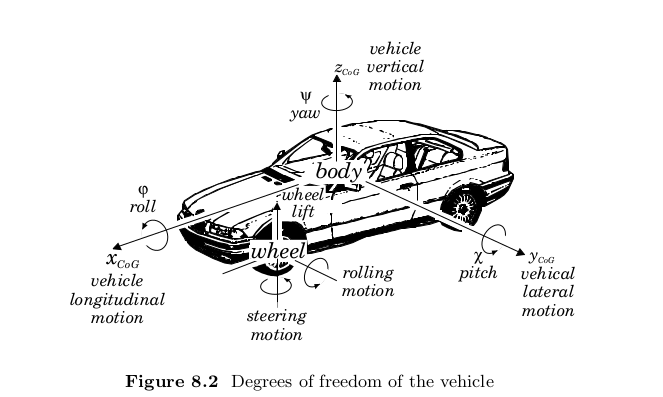
\includegraphics[width=\textwidth]{draft/stolen-figures/dof-vehicle.png}
    \caption{Degrees of freedom, vehicle}
    \label{fig:dof-vehicle}
\end{figure}

All coordinate systems, except the fixed inertial system, move during travel. The CoG has its origin at the vehicles center of gravity. The undercarriage lies centered at road level at a perpendicular projection from the rear axle. 
Each wheel has its own coordinate system. In \cite{kiencke}, the rear wheels coordinate direction are the same as the undercarriage system. For the front wheels only the wheel turn angle is different. See \cref{fig:dof-vehicle}.

\begin{table}
    \centering
    \begin{tabularx}{\linewidth}{|l|L|}
    \hline
     $x_{CoG}, y_{CoG}, z_{CoG}$ & Axis for the center of gravity coordinate system \\
     $x_{Un}, y_{Un}, z_{Un}$ & Axis for the undercarriage coordinate system \\
     $x_{W}, y_{W}, z_{W}$ & Axis for the wheel coordinate system. F and R denote front and rear, R and L denote right and left, so $x_{WRL}$ would be x-direction for rear left wheel. \\
     $x_{In}, y_{In}, z_{In}$ &  Axis for inertial coordinate system \\
     $\psi$ & Yaw angle (rotation about $z_{CoG}$) \\
     $\chi$ & Pitch angle (rotation about $y_{CoG}$) \\
     $\phi$ & Roll angle (rotation about $x_{CoG}$) \\
     $\alpha$ & Tire side slip angle (angle between $x_W$ and $v_W$, the wheel ground contact point velocity) \\
     $\delta_W$ & Wheel turn angle (angle between $x_{CoG}$ and $x_W$. Not the same as the steering angle $\delta_S$. \\
     $\beta$ & Vehicle body side slip angle (angle between $x_{CoG}$ and $v_{CoG}$, the vehicle velocity. \\ \hline
    \end{tabularx}
    \label{tab_coordinate_variables}
    \caption{Coordinate system variables}
\end{table}


\subsection{Wheel model}

Wheel forces are the most important forces in creating a simulation model for a motor vehicle. The wheel model is used for deriving the horizontal forces acting on the wheel. Need to know wheel slip, tire side slip angle and friction coefficients.

\begin{figure}
    \centering
    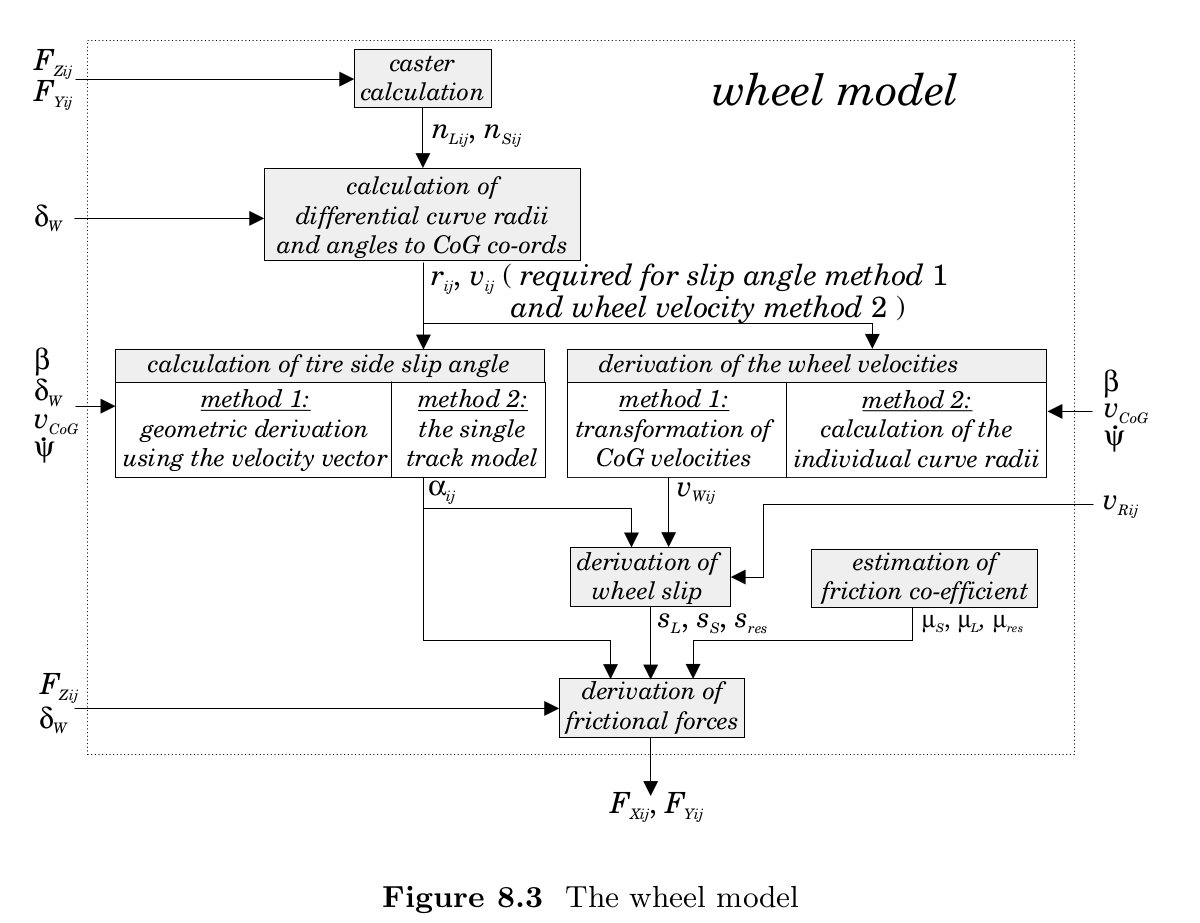
\includegraphics[width=\textwidth]{draft/stolen-figures/wheel-model.png}
    \caption{Wheel model overview}
    \label{fig:wheel-model}
\end{figure}

\paragraph{Method 1: Transformation of CoG velocity}

It is necessary to know the casters $n_L$ and $n_S$. These can be obtained from approximation formula citation 12 in \cite{kiencke}.

\begin{equation}
    n_L = \frac{1}{2}\left( l_0 + l_1\frac{F_Z}{F_{Z0}} \right)
    \quad \text{and} \quad 
    n_S = 3 n_L \tan{\alpha} + \frac{F_Y}{c_\text{press}}
\end{equation}

$n_L$ is known as the dynamic caster 

\info[inline]{looking at autoagri drawings, it looks like the caster is close to zero. This means the controller needs to ensure directional stability of the wheels, but it also may simplify some expressions.}

Wheel ground contact velocities equation (8.4 from \cite{kiencke}).

\begin{align*}
    \vector{v}_{WFL} &= \left( v_{CoG} \cos{\beta} - \dot{\phi} r_{FL} \sin{\theta_{FL}} \right) \unitvector{X}  +  \left( v_{CoG} \sin{\beta} + \dot{\phi} r_{FL} \cos{\theta_{FL}} \right) \unitvector{Y} \\
    \vector{v}_{WFR} &= \left( v_{CoG} \cos{\beta} + \dot{\phi} r_{FR} \cos{\theta_{FR}} \right) \unitvector{X}  +  \left( v_{CoG} \sin{\beta} + \dot{\phi} r_{FR} \sin{\theta_{FL}} \right) \unitvector{Y} \\
    \vector{v}_{WRL} &= \left( v_{CoG} \cos{\beta} - \dot{\phi} r_{RL} \cos{\theta_{RL}} \right) \unitvector{X}  +  \left( v_{CoG} \sin{\beta} - \dot{\phi} r_{RL} \sin{\theta_{FL}} \right) \unitvector{Y} \\
    \vector{v}_{WRR} &= \left( v_{CoG} \cos{\beta} + \dot{\phi} r_{RR} \sin{\theta_{RR}} \right) \unitvector{X}  +  \left( v_{CoG} \sin{\beta} - \dot{\phi} r_{RR} \cos{\theta_{RR}} \right) \unitvector{Y}
\end{align*}



\cite{kiencke} gives 2 methods for determining wheel velocities, but states that method 1 must be used when the wheel side slip angle is to be derived individually for all four wheels (See section 8.3.2 in \cite{kiencke}).

\subsection{Wheel slip and tire side slip angle}    


Assuming the method above was used to calculate the wheel velocities, it is straight forward to compute wheel sideslip. Look at \cref{fig:wheel-sideslip}. 

\begin{figure}
    \centering
    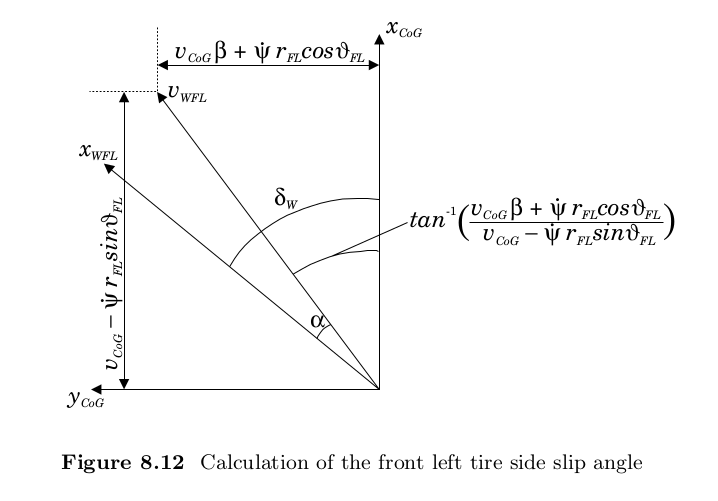
\includegraphics[width=\textwidth]{draft/stolen-figures/wheel-sideslip.png}
    \caption{Sideslip}
    \label{fig:wheel-sideslip}
\end{figure}

For a two-track vehicle the front wheels have the same steering angle $\delta_W$, but this is straight forward to generalize to a vehicle with independent steering angles on each wheel.

\todo[inline]{check the sign on these expressions by making a figure. Right now it is most likely incorrect.}
\begin{align*}
    \alpha_{FL} &= \delta_{WFL} - \arctan{\frac{v_{WFL,y}}{v_{WFL,x}}} \\
    \alpha_{FR} &= \pm \delta_{WFR} \pm  \arctan{\frac{v_{WFR,y}}{v_{WFR,x}}} \\
    \alpha_{RL} &= \pm \delta_{WRL} \pm \arctan{\frac{v_{WRL,y}}{v_{WRL,x}}} \\
    \alpha_{RR} &= \pm \delta_{WRR} \pm \arctan{\frac{v_{WRR,y}}{v_{WRR,x}}}
\end{align*}



\subsection{Friction coefficient calculation}

We want to model the friction force with slip. 
Burckhardt approach.
\begin{equation}
    \mu(s_{Res}) = c_1 \left( 1 - e^{-c_2 s_{Res}} \right) - c_r s_{Res}
\end{equation}

$s_{Res}$ is the resultant slip. Slip can occur in both longitudinal and lateral directions, so the friction $\mu_{Res}$ can be split into two parts.
\begin{equation}
    
\end{equation}